\documentclass[a4paper, 11pt]{article}

\usepackage[utf8]{inputenc}
\usepackage[T1]{fontenc}
\usepackage[francais]{babel} 
\usepackage{amsmath} % pour les formules de maths
\usepackage{amssymb} % pour des symboles
\usepackage{mathrsfs} % pour avoir acces a des jolies lettres calligrafiées. :)
\usepackage{listings} % pour le code source
\usepackage{color} % pour les couleurs
\usepackage{graphicx} % pour les graphiques (images)
\usepackage{fancyhdr} % pour utiliser le pagestyle fancy
\usepackage[headheight=14pt]{geometry} % pour les marges
\usepackage{hyperref}

\geometry{hmargin=3cm}

\title{Projet de Master}
\author{Romain Mencattini}
\date{\today}

\pagestyle{fancy} % pour avoir des entetes et des pieds de page
\renewcommand\headrulewidth{0.6pt}
\fancyhead[L]{Romain Mencattini} % haut de page gauche
\fancyhead[R]{Université de Genève \today} % haut de page droite

\begin{document}
\maketitle
\newpage
\tableofcontents
\newpage

%%%%%%%%%%%%%%%%%%%%%%%%%%%%%%%%%%%%%%%%%%%%%%%%%%%%%%%%%%%%%%%%%%%%%%%%%%
% début de l'état de l'art %%%%%%%%%%%%%%%%%%%%%%%%%%%%%%%%%%%%%%%%%%%%%%%
%%%%%%%%%%%%%%%%%%%%%%%%%%%%%%%%%%%%%%%%%%%%%%%%%%%%%%%%%%%%%%%%%%%%%%%%%%
\section{État de l'art}
\subsection{Introduction}
\paragraph{}
Avant la démocratisation de l'informatique et de son utilisation, toutes les opérations financières étaient réalisées par des humains. Ce système pouvait avoir des inconvénients :
\begin{itemize}
\item L'émotionnel pouvait influer les transactions. En effet, ces dernières étant effectuées par des humains, il y avait une risque non négligeable que l'état de la personne agisse sur sa décision.
\item Un problème sous-jacent était de maintenir une discipline de \textit{trading}. Afin de minimiser les pertes et de maximiser les gains, il fallait se tenir à ce plan afin de ne pas ce laisser influencer par des paramètres extérieurs. Cela pouvait être très difficile.
\item Le \textit{backtesting}\footnote{Backtesting is the process of testing a trading strategy on relevant historical data to ensure its viability before the trader risks any actual capital. $[$ \ref{backtesting investopedia} $]$} était impossible. Tester la qualification ainsi que la qualité de \textit{trading} d'une personne était compliquée. De même pour un \textit{trading plan}.
\end{itemize}

\paragraph{}
Ces éléments ont, en partie, favorisé l'émergence et l'utilisation d'algorithmes dans la finance. En 2014 aux USA, 84\% des transactions étaient accomplies par des algorithmes.\footnote{Financial Times : $[$ \ref{real investors} $]$} Ce qui représente environ 100000 réalisations, ou \textit{ticks}, par secondes. \footnote{Financial Times : $[$ \ref{real investors} $]$}
De part l'utilisation intensive de cet outil informatique, le monde de la finance a suivi l'évolution de ce domaine. Afin de perfectionner leurs algorithmes.
On retrouve donc des méthodes d'optimisations poussées ainsi que les récentes découvertes de \textit{data mining} et de \textit{machine learning}, abrégé \textit{ML}. Des propositions de plus en poussées dans les deux domaines voient le jour. L'algorithme qui sera au coeur de ce projet en fait partie. Il s'agit d'un réseau de neurones avec plusieurs couches prenant en compte des paramètres particuliers à la finance.

\paragraph{}Afin d'approcher aux mieux ces notions, nous allons discuter des éléments nécessaires à la compréhension.
Nous allons en premier lieu introduire le domaine financier ainsi que ces outils. Puis nous parlerons de plusieurs méthodes de \textit{ML}.
Voici celles vont être développées dans cet état de l'art :
\begin{itemize}
\item Les réseaux de neurones.
\item Les arbres de décision.
\item Les algorithmes \textit{SVM}\footnote{ Article \textit{SVM}: $[$ \ref{wikipedia svm} $]$}.
\item \textit{Logistic Regression}.
\item \textit{Naive Bayes}.
\item Descente du Gradient\footnote{Article Wikipedia : $[$ \ref{wikipedia descente du gradient} $]$} ainsi que sa version dite stochastique\footnote{Article parlant du gradient stochastique : $[$ \ref{descente du gradient stochastique} $]$}.
\end{itemize}

Finalement, nous lierons les deux domaines en montrant comment adapter les modèles mathématiques de \textit{ML} pour les utiliser comme techniques de \textit{trading}.


\subsection{Finance}
\subsubsection{Introduction}
\paragraph{}
Dans la partie Finance, nous allons traiter deux points :
\begin{enumerate}
\item Les différents types de marchés utilisés dans les articles.
\item Les outils relatifs à la finance.
\end{enumerate}

\subsubsection{Marchés}
\paragraph{}Les deux principaux marchés présents dans les articles utilisés sont :
\begin{itemize}
\item \textit{FOREX}
\item \textit{Stock Market}
\end{itemize}

\paragraph{}
Le marché \textit{FOREX} porte sur les devises. La valeur d'une devise doit être exprimée en fonction d'une autre. Il ne peut être dit qu'un franc suisse vaut 10. Il faut l'exprimer comme 1 franc suisse vaut 1.05 euro.\footnote{Taux fictif utilisé pour l'exemple.}
La transaction porte donc sur deux monnaies par exemple CHF/EUR\footnote{Franc Suisse - Euro} ou CHF/USD\footnote{Franc Suisse - Dollar Américain}. On va vendre des francs suisses pour acheter des dollars ou vendre des euros et acheter des franc suisses.
Le nom du marché vient d'ailleurs de ces échanges. On échange une monnaie contre une autre, c'est un \textit{FOreign EXchange}, ou \textit{FOREX}.

Les prix proviennent de l'offre et la demande. Comme illustration récente, on peut citer le cas de la Suisse. Le CHF étant jugé plus sûr, par le marché, que l'EUR, son prix a augmenté par rapport à l'EUR. Car la demande était importante. On peut également mentionner que même si les marchés peuvent être corrélés, il peut y avoir des différences. Par exemple\footnote{Source des images : $[$ \ref{historique taux de change} $]$}: \paragraph{}
\newpage
\begin{figure}[!htb]
\centering
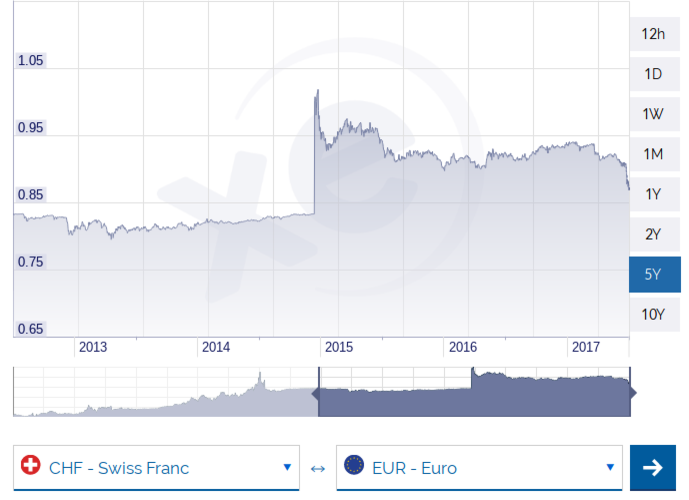
\includegraphics[scale=0.35]{images/chf_eur_5ans}
\caption{Cours CHF/EUR de 2013 à 2017}
\end{figure}

\begin{figure}[!htb]
\centering
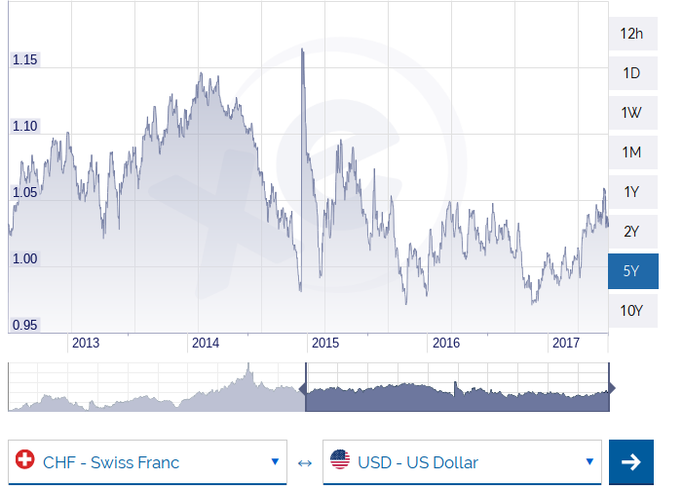
\includegraphics[scale=0.35]{images/chf_usd_5ans}
\caption{Cours CHF/USD de 2013 à 2017}
\end{figure}

\paragraph{}
On peut observer qu'en fin 2014, début 2015, le CHF a pris de la valeur par rapport à l'EUR et l'USD. Mais qu'ensuite le CHF a été dévalué par rapport à l'USD alors qu'il est resté stable par rapport à l'EUR.
Il peut donc y avoir corrélation comme en fin 2014, début 2015, mais les marchés des devises ne sont pas forcément liés.

\paragraph{}
La mondialisation a facilité ce marché. En effet, toutes les devises sont accessibles depuis n'importe où. Il devient donc possible d'avoir des marchés avec des devises plus exotiques.

Les principaux outils financiers utilisés sont les options. Nous 

\subsection{Cadre théorique des algorithmes de \textit{Machine Learning}}
\subsection{\textit{Machine Learning} dans le cadre de la finance}
\subsection{Conclusion}
\newpage
%%%%%%%%%%%%%%%%%%%%%%%%%%%%%%%%%%%%%%%%%%%%%%%%%%%%%%%%%%%%%%%%%%%%%%%%%%
% début du projet  %%%%%%%%%%%%%%%%%%%%%%%%%%%%%%%%%%%%%%%%%%%%%%%%%%%%%%%
%%%%%%%%%%%%%%%%%%%%%%%%%%%%%%%%%%%%%%%%%%%%%%%%%%%%%%%%%%%%%%%%%%%%%%%%%%
\section{Projet}
\newpage
%%%%%%%%%%%%%%%%%%%%%%%%%%%%%%%%%%%%%%%%%%%%%%%%%%%%%%%%%%%%%%%%%%%%%%%%%%
% début de la bibliographie %%%%%%%%%%%%%%%%%%%%%%%%%%%%%%%%%%%%%%%%%%%%%%
%%%%%%%%%%%%%%%%%%%%%%%%%%%%%%%%%%%%%%%%%%%%%%%%%%%%%%%%%%%%%%%%%%%%%%%%%%
\section{Bibliographie}

\begin{enumerate}
\item Financial Times : "\textit{Real investors eclipsed by fast trading}", 2012 \url{https://www.ft.com/content/da5d033c-8e1c-11e1-bf8f-00144feab49a?mhq5j=e1} \label{real investors}
\item "\textit{A Machine Learning Approach to Automated Trading}", 09.05.2016, Ning Lu
\item "\textit{An efficient implementation of the backtesting of trading strategies.}" Ni, Jiarui, et Chegqi Zhang, \textit{Parallel and Distributed Processing and Applications} (2005): 126-131.
\item "\textit{Algorithmic Trading: Winning Strategies and Their Rationale ( Wiley Trading Series)}", John Wiley and Sons, 2013
\item "\textit{Machine Learning}", Mitchell, Tom M. New York, 1997.
\item Article Wikipédia sur SVM : \url{https://fr.wikipedia.org/wiki/Machine_\%C3\%A0_vecteurs_de_support} \label{wikipedia svm}
\item "\textit{Online Machine Learning Algorithms For Currency Exchange Prediction}", Eleftherios Soulas et Dennis Shasha de NYU, Courant Department. \label{descente du gradient stochastique}
\item  Article Wikipédia sur Algorithme du gradient : \url{https://fr.wikipedia.org/wiki/Algorithme_du_gradient} \label{wikipedia descente du gradient}
\item "\textit{Descision Tree Learning}", Tom M. Mitchell
\item Article Investopedia sur les Options \url{http://www.investopedia.com/terms/o/option.asp}
\item "\textit{Support Vector Machine (and Statistical Learning Theory) Tutorial}", de Jason Weston, NEC Labs America. \url{http://www.cs.columbia.edu/~kathy/cs4701/documents/jason_svm_tutorial.pdf}
\item  "\textit{An Introduction to Neural Networks}" Vincent Cheung et Kevin Cannons : \url{http://www2.econ.iastate.edu/tesfatsi/NeuralNetworks.CheungCannonNotes.pdf}
\item Exemple de réseaux de neurones\url{http://csc.lsu.edu/~jianhua/nn.pdf} p.5
\item \textit{Backtesting} Investopedia \url{http://www.investopedia.com/terms/b/backtesting.asp} \label{backtesting investopedia}
\item Historique des taux de changes : \url{http://www.xe.com/currencycharts/} \label{historique taux de change}
\end{enumerate}


\end{document}